\section{Espesor de la coroides: resto de imágenes}
Debido a la gran cantidad de imágenes utilizadas en este trabajo, sólo
se han añadido al apéndice una mínima selección correspondiente al
estudio de un único paciente junto a los resultados obtenidos. El
resto de imágenes se proporcionan en el CD adjunto.
\begin{figure}[H]
  \caption{Original}
  \centering \setlength\fboxsep{0pt} \setlength\fboxrule{0.5pt}
  \fbox{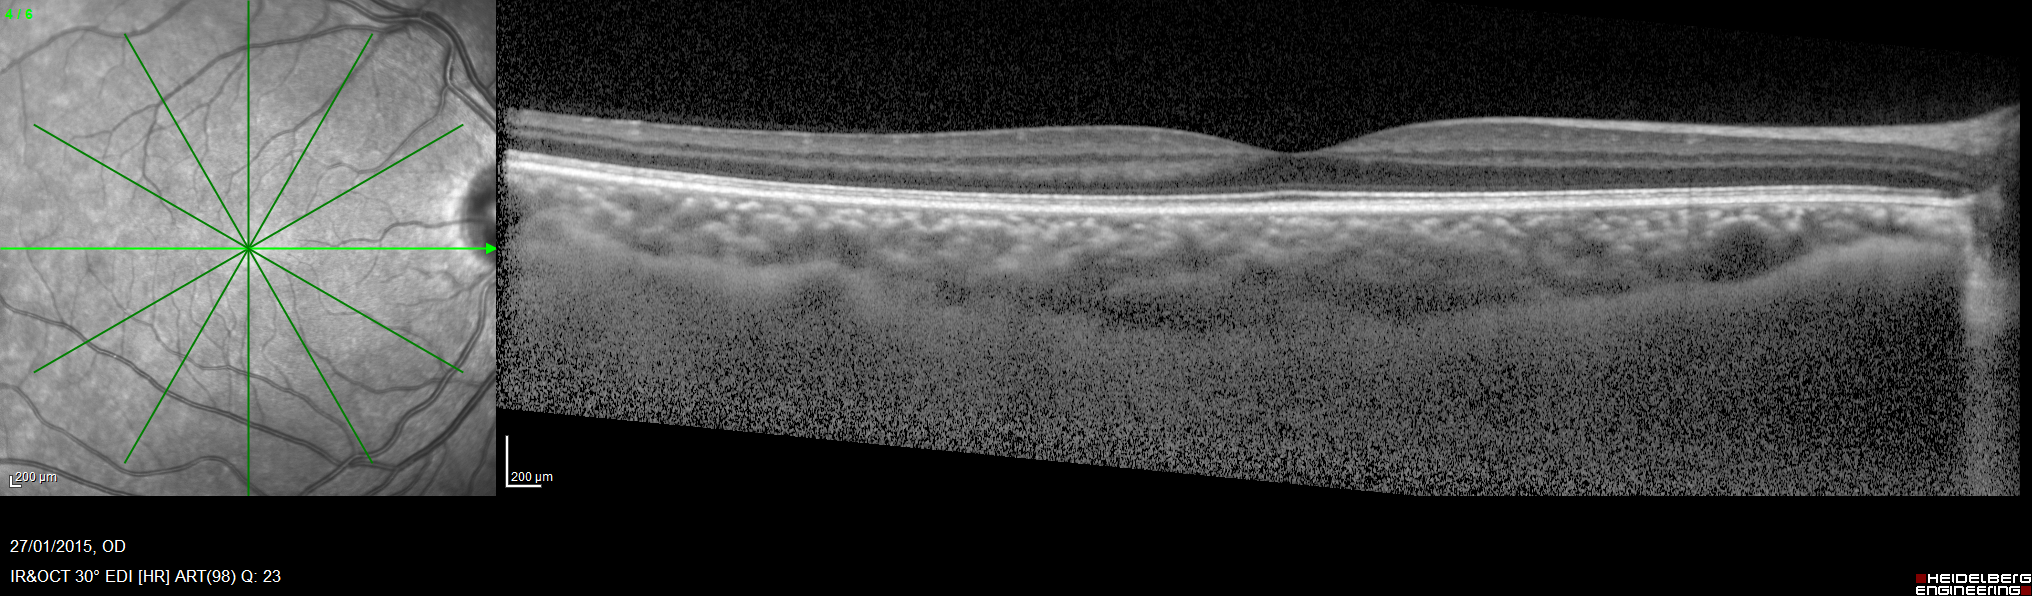
\includegraphics[width=\textwidth]{imagenes/apendices/A_D2.png}}
\end{figure}

\begin{figure}[H]
  \caption{Procesada}
  \centering \setlength\fboxsep{0pt} \setlength\fboxrule{0.5pt}
  \fbox{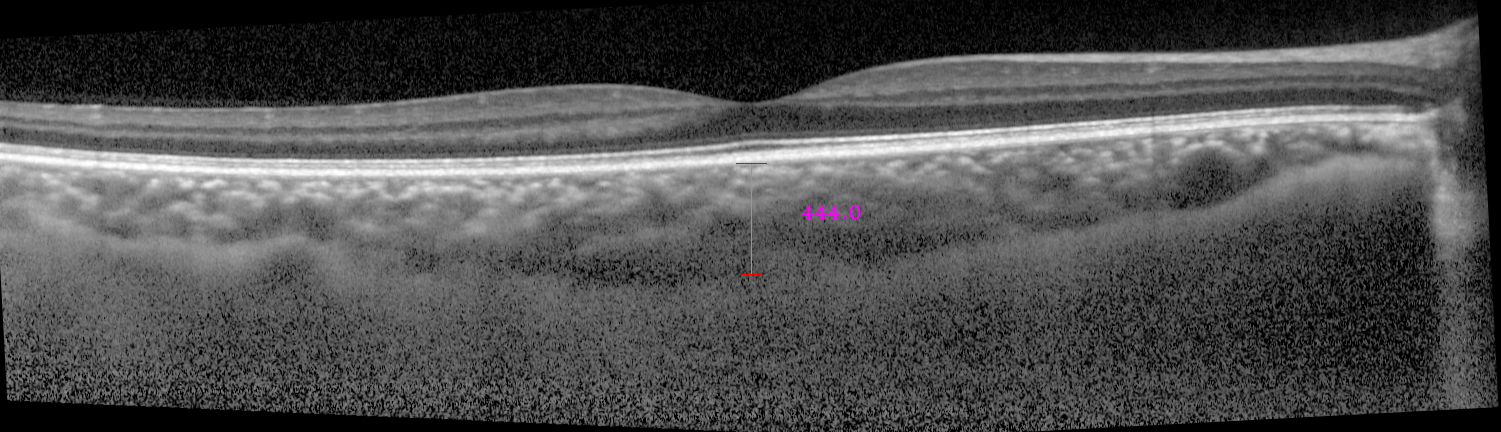
\includegraphics[width=\textwidth]{imagenes/apendices/PROCESADAS/A_D2_iteration=1_espesor_final.png}}
\end{figure}



\begin{figure}[H]
  \caption{Original}
  \centering \setlength\fboxsep{0pt} \setlength\fboxrule{0.5pt}
  \fbox{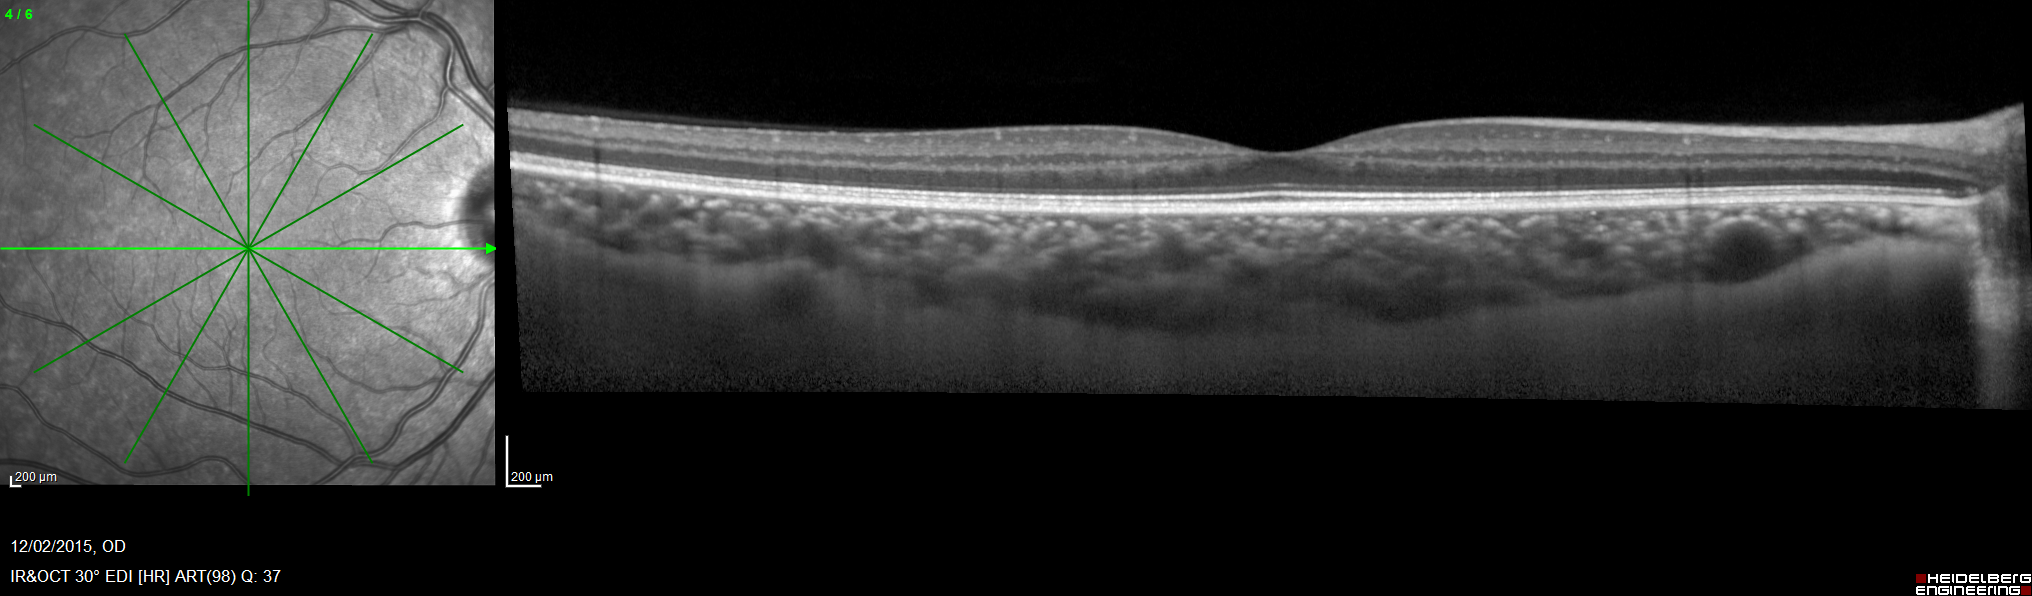
\includegraphics[width=\textwidth]{imagenes/apendices/A_D5.png}}
\end{figure}

\begin{figure}[H]
  \caption{Procesada}
  \centering \setlength\fboxsep{0pt} \setlength\fboxrule{0.5pt}
  \fbox{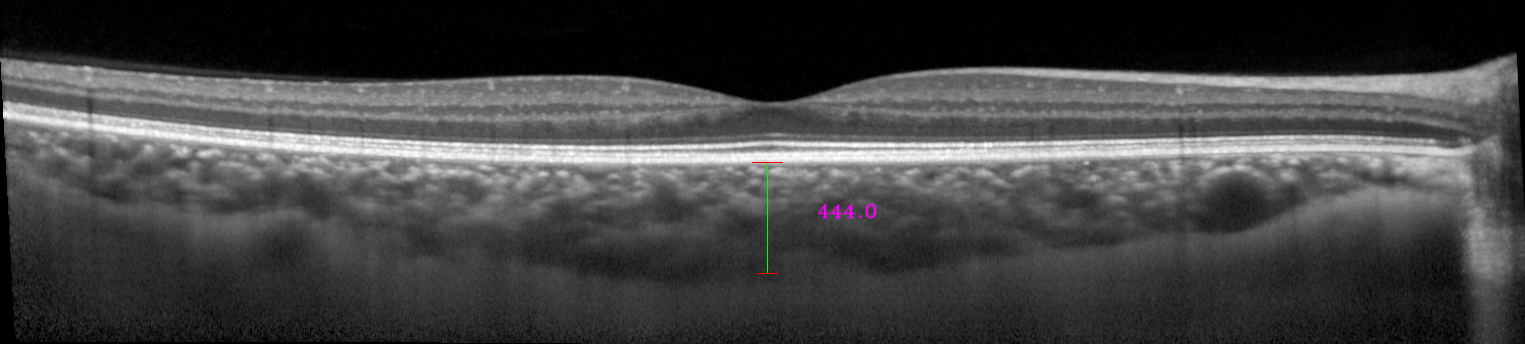
\includegraphics[width=\textwidth]{imagenes/apendices/PROCESADAS/A_D5_iteration=1_espesor_final.png}}
\end{figure}


\begin{figure}[H]
  \caption{Original}
  \centering \setlength\fboxsep{0pt} \setlength\fboxrule{0.5pt}
  \fbox{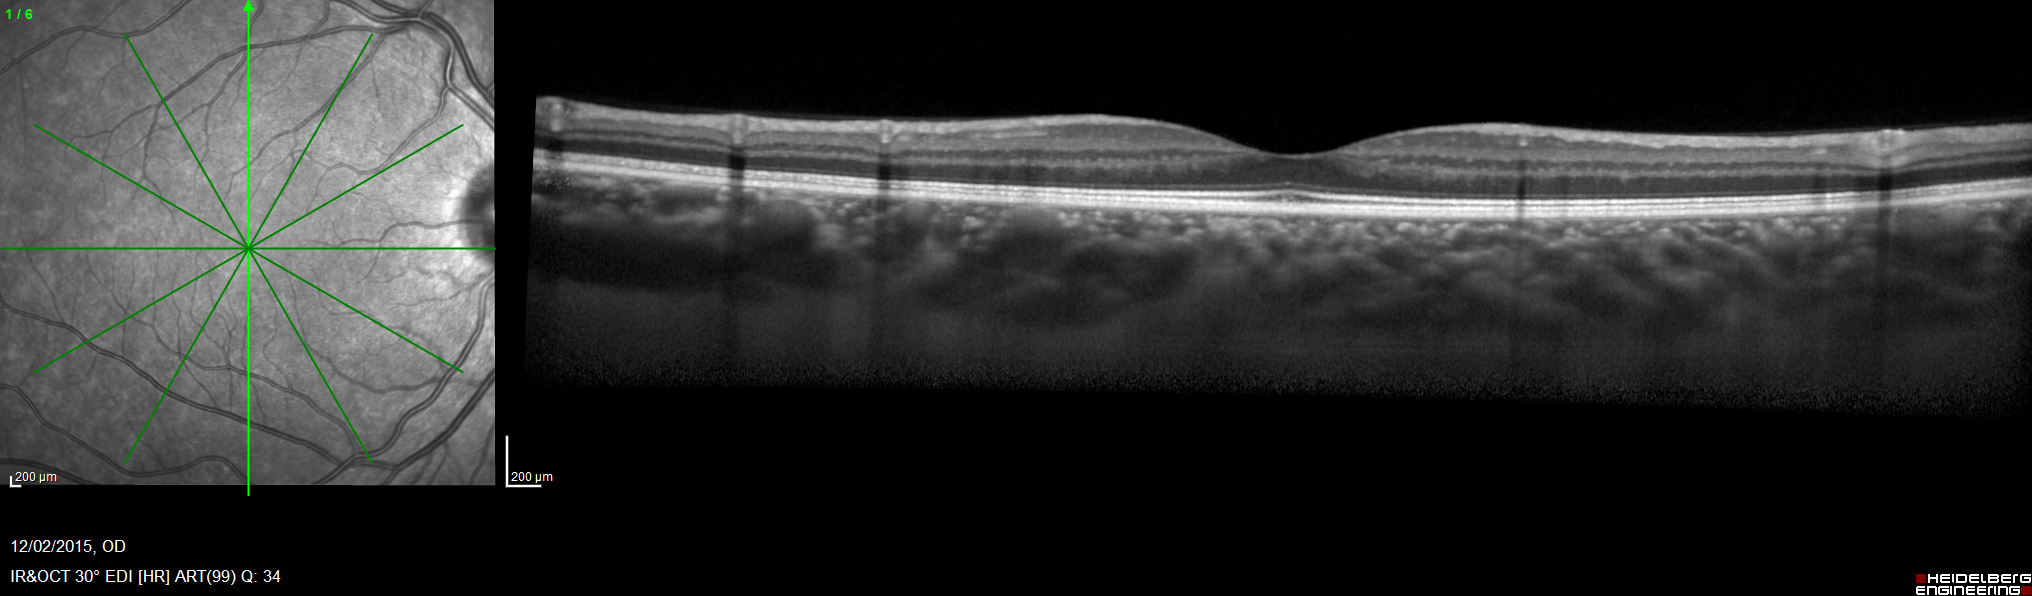
\includegraphics[width=\textwidth]{imagenes/apendices/A_D6.png}}
\end{figure}

\begin{figure}[H]
  \caption{Procesada}
  \centering \setlength\fboxsep{0pt} \setlength\fboxrule{0.5pt}
  \fbox{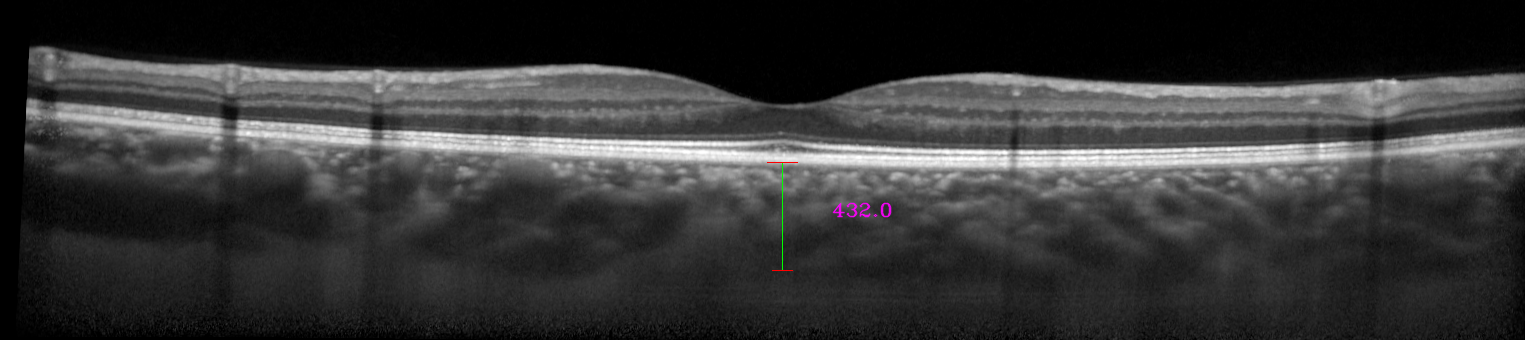
\includegraphics[width=\textwidth]{imagenes/apendices/PROCESADAS/A_D6_iteration=1_espesor_final.png}}
\end{figure}
